%photoshop
\subsection{Changing and matching skin colour in Photoshop}

Skin colour correction is a frequently encountered problem in photo retouching and there are a wide range of online video tutorials available documenting the methods artists use to manually adjust human skin colour in individual images using Adobe Photoshop, a widely used commercial image manipulation software. The purposes of these videos include giving the subject of an image the appearance of a tan, matching the skin tone of the subject to a desired skin tone on another individual, or matching the skin tone of a subject's face to the rest of the subject's body, which is often a slightly different colour \cite{photoshop:tan, photoshop:match_other, photoshop:match_body}. Bearing in mind that techniques described by such tutorials expect artistic input from a human editor to achieve the results and are therefore not entirely applicable to the purpose of this project, it is useful to study these methods because the results achieved are usually extremely realistic and aesthetically pleasing and should be a standard that the algorithm developed for this project is designed towards. We therefore surveyed a number of these videos and summarize below the techniques of some of the most relevant tutorials.

\subsubsection*{Summary of Photoshop techniques}

Shaver demonstrated how to change a person's skin colour from dark to light \cite{photoshop:obama}. Shaver used levels and curves, which are tools that manipulate the $RGB$ colour histogram of the image, to increase brightness to an extent, then performed further brightening by using a grey scale conversion to brighten the skin area of a black and white image and then using the luminosity blend mode to place the colour back into the image. We show the results achieved in Table \ref{tab:obama_demo}.

\begin{table}[H]
    \centering
    \caption{Screen captures from Shaver's Photoshop tutorial for changing skin colour from dark to light \cite{photoshop:obama}. \label{tab:obama_demo}}
\begin{tabular}{|c|c|}
    \hline
    Source & Output \\
    \hline
  \begin{minipage}{.29\textwidth}
    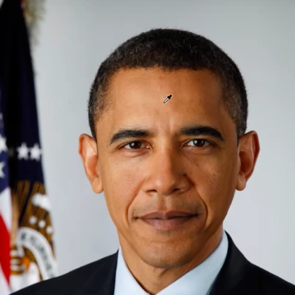
\includegraphics[width=\textwidth,height=\textheight,keepaspectratio]{images/obama_orig}
  \end{minipage} & 
  \begin{minipage}{.29\textwidth}
    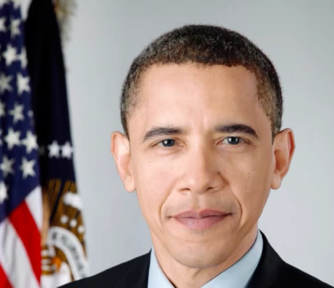
\includegraphics[width=\textwidth,height=\textheight,keepaspectratio]{images/obama_res}
  \end{minipage} \\
    \hline
\end{tabular}
\end{table}

Phlearn demonstrated an effect in the reverse direction by demonstrating a technique for giving the model the appearance of a dark tan \cite{photoshop:tan}. The highlights and shadows of the image are adjusted separately by using the ``blend if" function of Photoshop, which blends in an effect only if the original pixel is above or below a certain threshold of brightness.

Phlearn also demonstrated a method for matching the skin colour of body and face in an image where the two appear mismatched \cite{photoshop:match_body}. The author sampled a range of colours from the body and adjusted the face with the levels tool for each colour channel. We show the results achieved in Table \ref{tab:match_body_demo}.

\begin{table}[H]
    \centering
    \caption{Screen captures from Photoshop tutorial for matching the skin tones of face and body. \label{tab:match_body_demo}}
\begin{tabular}{|c|c|c|}
    \hline
    Source & Target & Output \\
    \hline
  \begin{minipage}{.29\textwidth}
    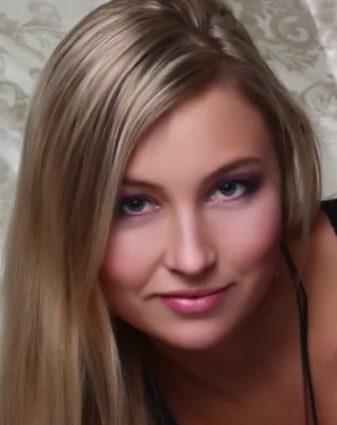
\includegraphics[width=\textwidth,height=\textheight,keepaspectratio]{images/match_body_orig}
  \end{minipage} & 
  \begin{minipage}{.29\textwidth}
    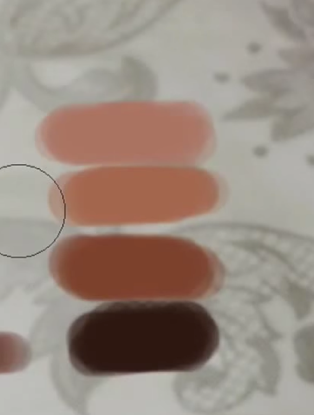
\includegraphics[width=\textwidth,height=\textheight,keepaspectratio]{images/match_body_targ}
  \end{minipage} & 
  \begin{minipage}{.29\textwidth}
    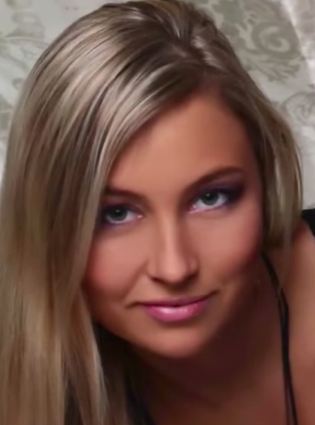
\includegraphics[width=\textwidth,height=\textheight,keepaspectratio]{images/match_body_res}
  \end{minipage} \\
    \hline
\end{tabular}
\end{table}

PiXimperfect demonstrated a method for matching skin colour in one portrait to another \cite{photoshop:match_other}. PiXimperfect first calculated the two average colours of the faces and then used the Photoshop curves tool to match the average colours of the original image to the target image. There must then be further adjustments by eye to change colour, brightness and contrast. Examples of the results from PiXimperfect is show in Table \ref{tab:match_other_demo}

\begin{table}[H]
    \centering
    \caption{Screen captures from Photoshop tutorial for matching the skin tones of portraits of different people. \label{tab:match_other_demo}}
\begin{tabular}{|c|c|c|}
    \hline
    Source & Target & Output \\
    \hline
  \begin{minipage}{.29\textwidth}
    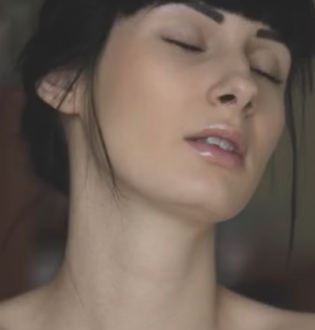
\includegraphics[width=\textwidth,height=\textheight,keepaspectratio]{images/match_other_1_orig}
  \end{minipage} & 
  \begin{minipage}{.29\textwidth}
    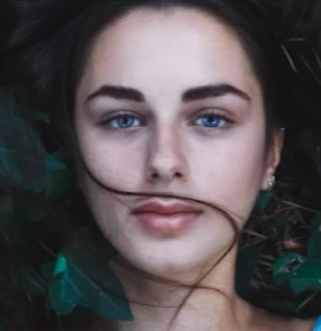
\includegraphics[width=\textwidth,height=\textheight,keepaspectratio]{images/match_other_1_targ}
  \end{minipage} & 
  \begin{minipage}{.29\textwidth}
    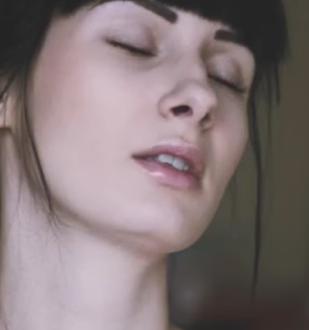
\includegraphics[width=\textwidth,height=\textheight,keepaspectratio]{images/match_other_1_res}
  \end{minipage} \\
    \hline
  \begin{minipage}{.29\textwidth}
    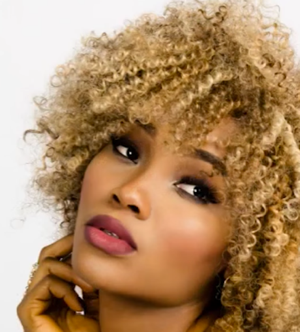
\includegraphics[width=\textwidth,height=\textheight,keepaspectratio]{images/match_other_2_orig}
  \end{minipage} & 
  \begin{minipage}{.29\textwidth}
    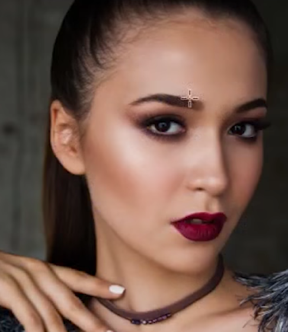
\includegraphics[width=\textwidth,height=\textheight,keepaspectratio]{images/match_other_2_targ}
  \end{minipage} & 
  \begin{minipage}{.29\textwidth}
    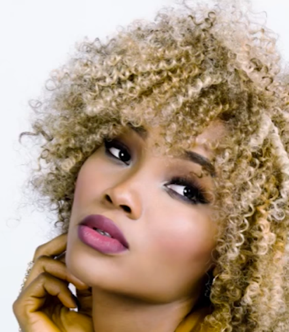
\includegraphics[width=\textwidth,height=\textheight,keepaspectratio]{images/match_other_2_res}
  \end{minipage} \\
    \hline
\end{tabular}
\end{table}

Generally, for most of the techniques surveyed, levels and curves are used for small brightness adjustments \cite{photoshop:obama, photoshop:match_body, photoshop:match_other}, and often to reduce the vividness of the colour adjustments the saturation must be slightly decreased \cite{photoshop:obama, photoshop:match_body}. After all other effects are applied, the opacity of the overall effect is often reduced from 100\% for a more natural appearance \cite{photoshop:obama, photoshop:match_body}.

\subsubsection*{Limitations of Photoshop techniques}
The Photoshop techniques surveyed are not meant for automation; instead, they are meant to be tailored to each specific image that a human is adjusting, and there are many junctures where the specific numerical amount of an adjustment have to be judged by eye. While Photoshop has a method for automating processes to an extent using \textit{actions} \cite{photoshop:actions}, the processes are meant for increasing ease of use by artists who can make additional adjustments and are familiar with the tool, rather than for use in commercial applications where the process is entirely automated.

Another limitation is that Photoshop operates at a higher level of abstraction than image processing code, which has much more control over processes that can be applied to images, and the regions on the image that processes are applied to. 

Finally, some Photoshop effects may be proprietary and are, of course, limited to the platforms that support Photoshop, while a program coded with image processing libraries can be made open source and can be integrated into applications running on a variety of different platforms.